\documentclass[../main.tex]{subfiles}
\graphicspath{{\subfix{../src/}}}


\begin{document}


\begin{figure}[h]
\begin{center}
\includegraphics[width=0.8\textwidth]{example-image-a}
\caption{Example figure text}
\label{fig:template}
\end{center}
\end{figure}

\begin{table}
\begin{center}
\begin{tabular}{ |l|l|c| } 
 \hline
 Grip Type & Finger Usage Description & ADL($\%$) \\ 
 \hline
 Pulp pinch & Between thumb, index and middle finger & 20 \\ 
 Lateral pinch & Between thumb \& side of index finger & 20 \\ 
 Five-Finger pinch & Between thumb, and all four fingers & 15 \\ 
 \hline
\end{tabular}
\caption{Example table}
\label{tab:??}
\end{center}
\end{table}

\end{document}




%TODO: this is not a good way to show results!
%\begin{figure}
%    \centering
%    \begin{subfigure}[b]{0.49\textwidth}
%        \centering
%        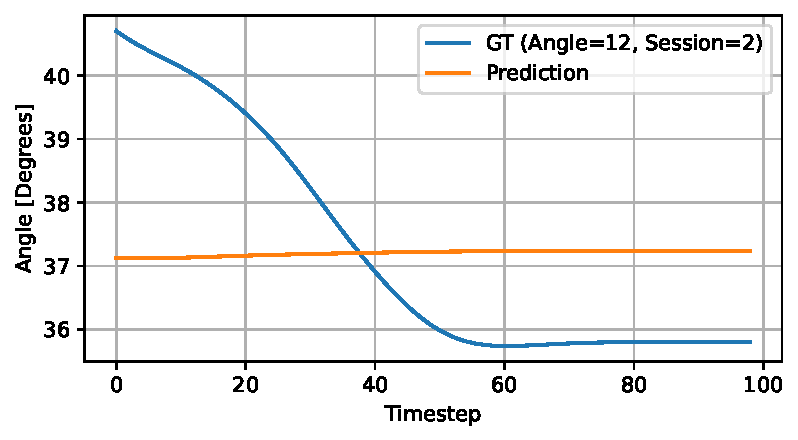
\includegraphics[width=\textwidth]{CNNtest0.pdf}
%        \caption{}
%        \label{fig:y equals x}
%    \end{subfigure}
%    \hfill
%    \centering
%    \begin{subfigure}[b]{0.49\textwidth}
%        \centering
%        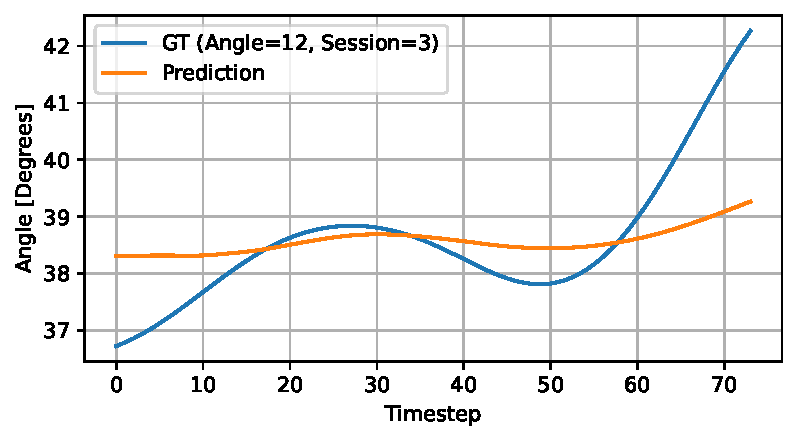
\includegraphics[width=\textwidth]{CNNtest1.pdf}
%        \caption{}
%        \label{fig:y equals x}
%    \end{subfigure}
%    \hfill
%    \begin{subfigure}[b]{0.49\textwidth}
%        \centering
%        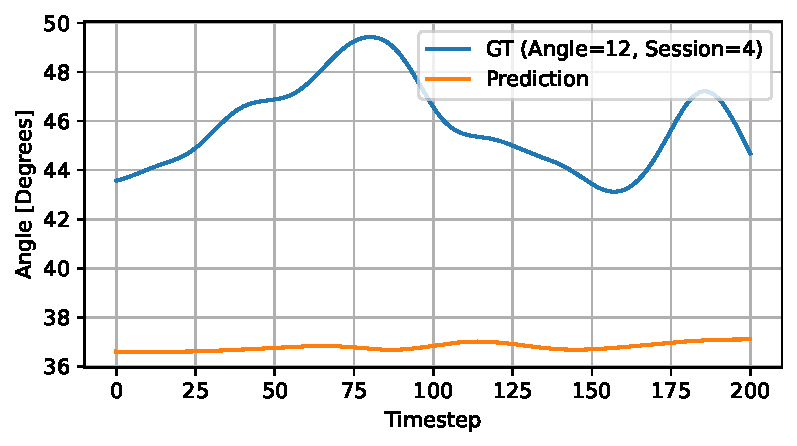
\includegraphics[width=\textwidth]{CNNtest2.pdf}
%        \caption{}
%        \label{fig:three sin x}
%    \end{subfigure}
%    \hfill
%    \begin{subfigure}[b]{0.49\textwidth}
%        \centering
%        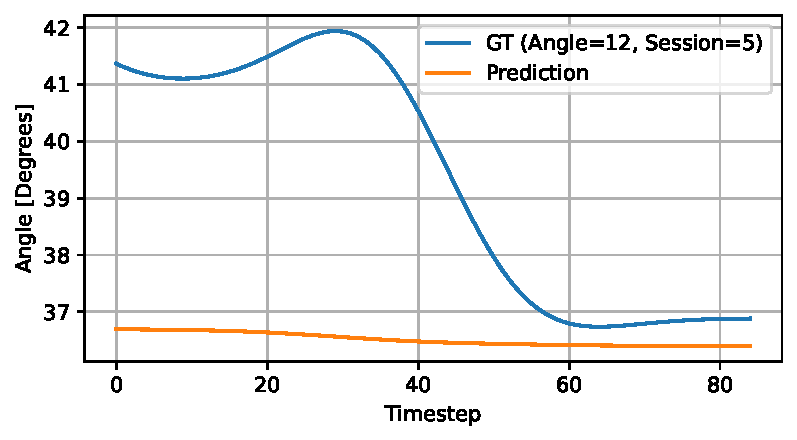
\includegraphics[width=\textwidth]{CNNtest3.pdf}
%        \caption{}
%        \label{fig:five over x}
%    \end{subfigure}
%    \hfill
%    \begin{subfigure}[b]{0.49\textwidth}
%        \centering
%        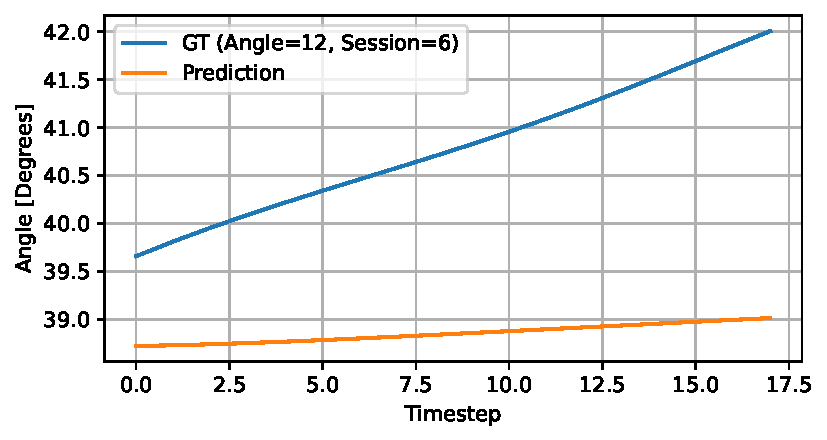
\includegraphics[width=\textwidth]{CNNtest4.pdf}
%        \caption{}
%        \label{fig:five over x}
%    \end{subfigure}
%    \hfill
%    \begin{subfigure}[b]{0.49\textwidth}
%        \centering
%        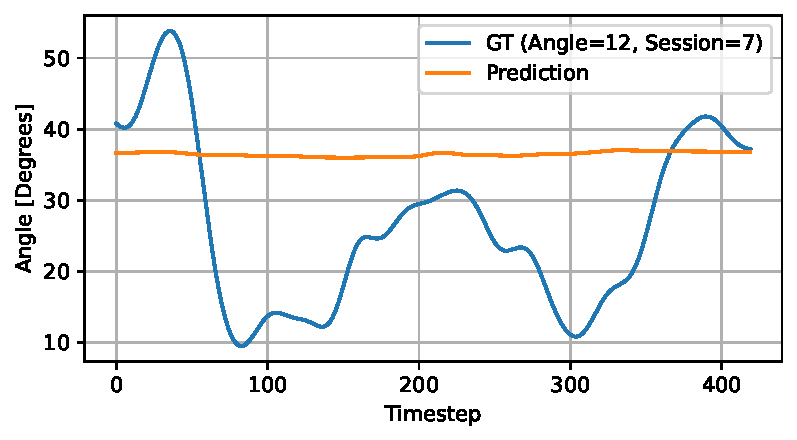
\includegraphics[width=\textwidth]{CNNtest5.pdf}
%        \caption{}
%        \label{fig:five over x}
%    \end{subfigure}
%    \hfill
%    \caption{Regression of Finger angles using a CNN network.}
%    \label{fig:CNNregression}
%\end{figure}



%\subsubsection{Pre-Processing Filters}
%\textbf{Method}\\
%\textbf{Test}\\
%\textbf{Results}\\
%
%\subsubsection{Window Size}
%\textbf{Method}\\
%\textbf{Test}\\
%\textbf{Results}\\
%
%\subsubsection{Training Parameters}
%\textbf{Method}\\
%\textbf{Test}\\
%\textbf{Results}\\
%
%\subsubsection{Types of Features for extraction}
%\textbf{Method}\\
%\textbf{Test}\\
%\textbf{Results}\\
%
%\subsection{3. Recurrent Neural Networks}
%
%\subsubsection{Training Parameters}
%\textbf{Method}\\
%\textbf{Test}\\
%\textbf{Results}\\
%


